\documentclass[border=6pt]{standalone}
\usepackage{tikz}
\usetikzlibrary{positioning,arrows.meta,shapes.geometric,fit,backgrounds,calc}
\usepackage[T1]{fontenc}
\usepackage{helvet}
\renewcommand{\familydefault}{\sfdefault}

\definecolor{ingest}{HTML}{E8F1FB}
\definecolor{ingestb}{HTML}{2E6DA4}
\definecolor{queue}{HTML}{FFF4E0}
\definecolor{queueb}{HTML}{B7791F}
\definecolor{worker}{HTML}{EAF5EC}
\definecolor{workerb}{HTML}{2F7D4F}
\definecolor{store}{HTML}{F1ECF7}
\definecolor{storeb}{HTML}{6B4C9A}
\definecolor{uifill}{HTML}{FDEBEC}
\definecolor{uib}{HTML}{A33A3A}
\definecolor{ink}{HTML}{1F2933}

\tikzset{
  box/.style 2 args={
    draw=#1, fill=#2, line width=0.7pt, rounded corners=3pt,
    align=center, text=ink, font=\scriptsize, inner sep=4pt,
    minimum height=0.95cm
  },
  flow/.style={-{Latex[length=2.2mm,width=1.6mm]}, line width=0.8pt, draw=ink!75},
  dashflow/.style={-{Latex[length=2.2mm,width=1.6mm]}, line width=0.7pt, draw=ink!55, dashed},
  label/.style={font=\scriptsize\bfseries, text=ink!80, align=left},
  band/.style={font=\scriptsize\bfseries, text=ink!55, align=center}
}

\begin{document}
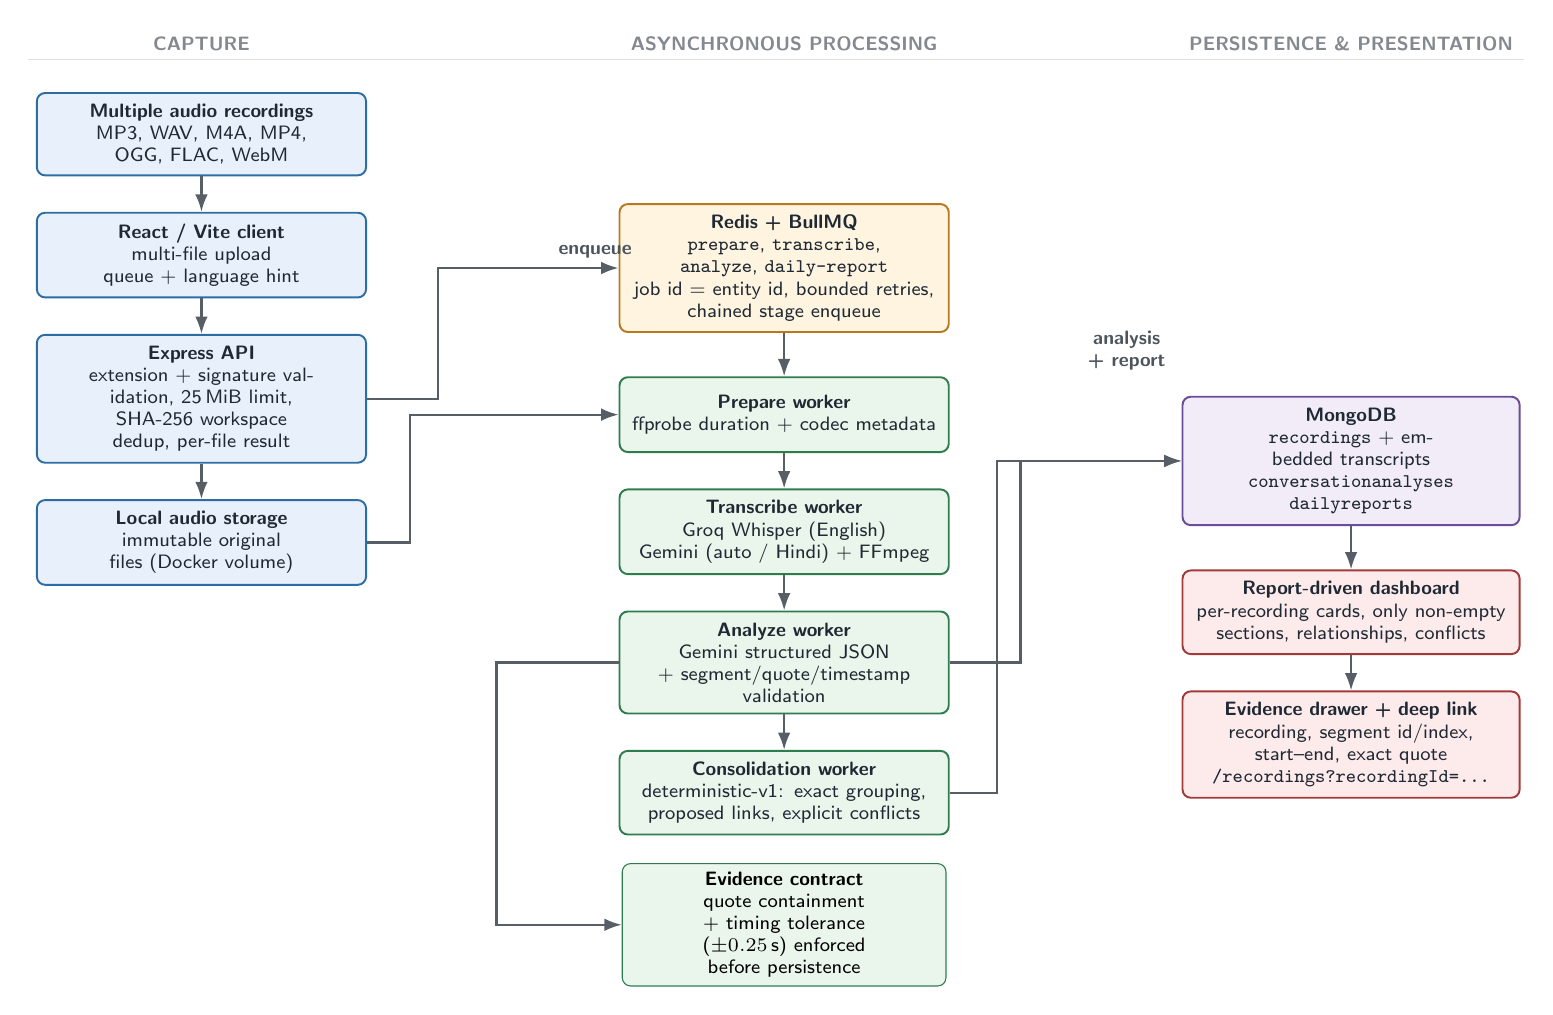
\begin{tikzpicture}[node distance=0.5cm and 0.6cm]

% ------------------------------------------------------------------ bands
\node[band] (b1) at (0,1.15) {CAPTURE};
\node[band] (b2) at (7.4,1.15) {ASYNCHRONOUS PROCESSING};
\node[band] (b3) at (14.6,1.15) {PERSISTENCE \& PRESENTATION};
\draw[ink!15, line width=0.4pt] (-2.2,0.95) -- (16.8,0.95);

% ------------------------------------------------------------------ capture
\node[box={ingestb}{ingest}, text width=3.9cm] (audio) at (0,0)
  {\textbf{Multiple audio recordings}\\ MP3, WAV, M4A, MP4, OGG, FLAC, WebM};
\node[box={ingestb}{ingest}, text width=3.9cm, below=0.45cm of audio] (web)
  {\textbf{React / Vite client}\\ multi-file upload queue + language hint};
\node[box={ingestb}{ingest}, text width=3.9cm, below=0.45cm of web] (api)
  {\textbf{Express API}\\ extension + signature validation, 25\,MiB limit,\\ SHA-256 workspace dedup, per-file result};
\node[box={ingestb}{ingest}, text width=3.9cm, below=0.45cm of api] (disk)
  {\textbf{Local audio storage}\\ immutable original files (Docker volume)};

% ------------------------------------------------------------------ queue
\node[box={queueb}{queue}, text width=3.9cm] (redis) at (7.4,-1.7)
  {\textbf{Redis + BullMQ}\\ \texttt{prepare}, \texttt{transcribe}, \texttt{analyze}, \texttt{daily-report}\\ job id = entity id, bounded retries,\\ chained stage enqueue};

% ------------------------------------------------------------------ worker
\node[box={workerb}{worker}, text width=3.9cm, below=0.55cm of redis] (prepare)
  {\textbf{Prepare worker}\\ ffprobe duration + codec metadata};
\node[box={workerb}{worker}, text width=3.9cm, below=0.45cm of prepare] (transcribe)
  {\textbf{Transcribe worker}\\ Groq Whisper (English)\\ Gemini (auto / Hindi) + FFmpeg};
\node[box={workerb}{worker}, text width=3.9cm, below=0.45cm of transcribe] (analyze)
  {\textbf{Analyze worker}\\ Gemini structured JSON\\ + segment/quote/timestamp validation};
\node[box={workerb}{worker}, text width=3.9cm, below=0.45cm of analyze] (consolidate)
  {\textbf{Consolidation worker}\\ deterministic-v1: exact grouping,\\ proposed links, explicit conflicts};

% ------------------------------------------------------------------ store
\node[box={storeb}{store}, text width=4.0cm] (mongo) at (14.6,-4.15)
  {\textbf{MongoDB}\\ \texttt{recordings} + embedded transcripts\\ \texttt{conversationanalyses}\\ \texttt{dailyreports}};

% ------------------------------------------------------------------ ui
\node[box={uib}{uifill}, text width=4.0cm, below=0.55cm of mongo] (dash)
  {\textbf{Report-driven dashboard}\\ per-recording cards, only non-empty\\ sections, relationships, conflicts};
\node[box={uib}{uifill}, text width=4.0cm, below=0.45cm of dash] (evidence)
  {\textbf{Evidence drawer + deep link}\\ recording, segment id/index,\\ start--end, exact quote\\ \texttt{/recordings?recordingId=\ldots}};

% ------------------------------------------------------------------ capture arrows
\draw[flow] (audio) -- (web);
\draw[flow] (web) -- (api);
\draw[flow] (api) -- (disk);

% ------------------------------------------------------------------ ingest -> queue
\draw[flow] (api.east) -- ++(0.9,0) |- (redis.west);
\node[label, above] at (5.0,-1.7) {enqueue};

% ------------------------------------------------------------------ queue -> worker
\draw[flow] (redis) -- (prepare);
\draw[flow] (prepare) -- (transcribe);
\draw[flow] (transcribe) -- (analyze);
\draw[flow] (analyze) -- (consolidate);

% ------------------------------------------------------------------ worker -> mongo
\draw[flow] (analyze.east) -- ++(0.9,0) |- (mongo.west);
\draw[flow] (consolidate.east) -- ++(0.6,0) |- (mongo.west);
\node[label, align=center] at (11.75,-2.75) {analysis\\ + report};

% ------------------------------------------------------------------ disk -> prepare
\draw[flow] (disk.east) -- ++(0.55,0) |- (prepare.west);

% ------------------------------------------------------------------ mongo -> ui
\draw[flow] (mongo) -- (dash);
\draw[flow] (dash) -- (evidence);

% ------------------------------------------------------------------ evidence contract
\node[draw=workerb, fill=worker, rounded corners=3pt, font=\scriptsize,
      align=center, text width=3.9cm, inner sep=3pt, below=0.35cm of consolidate]
  (contract) {\textbf{Evidence contract}\\ quote containment + timing tolerance\\ ($\pm0.25$\,s) enforced before persistence};
\draw[flow] (analyze.west) -- ++(-1.55,0) |- (contract.west);

\end{tikzpicture}
\end{document}
